\documentclass{article}
\usepackage{graphicx}
\usepackage{float}

\title{CMSC6950 Project Report: Tidynamics}
\author{Karina Barcelos}
\date{Spring - June 2021}

\setlength{\oddsidemargin}{0.5cm}
\setlength{\textwidth}{15.5cm}
\setlength{\topmargin}{-1.5cm}
\setlength{\textheight}{22cm}

\begin{document}
\maketitle

\section{Introduction}

Text 


\section{Results}

Text

\subsection{Task 1}

Text 

\begin{figure}[H]
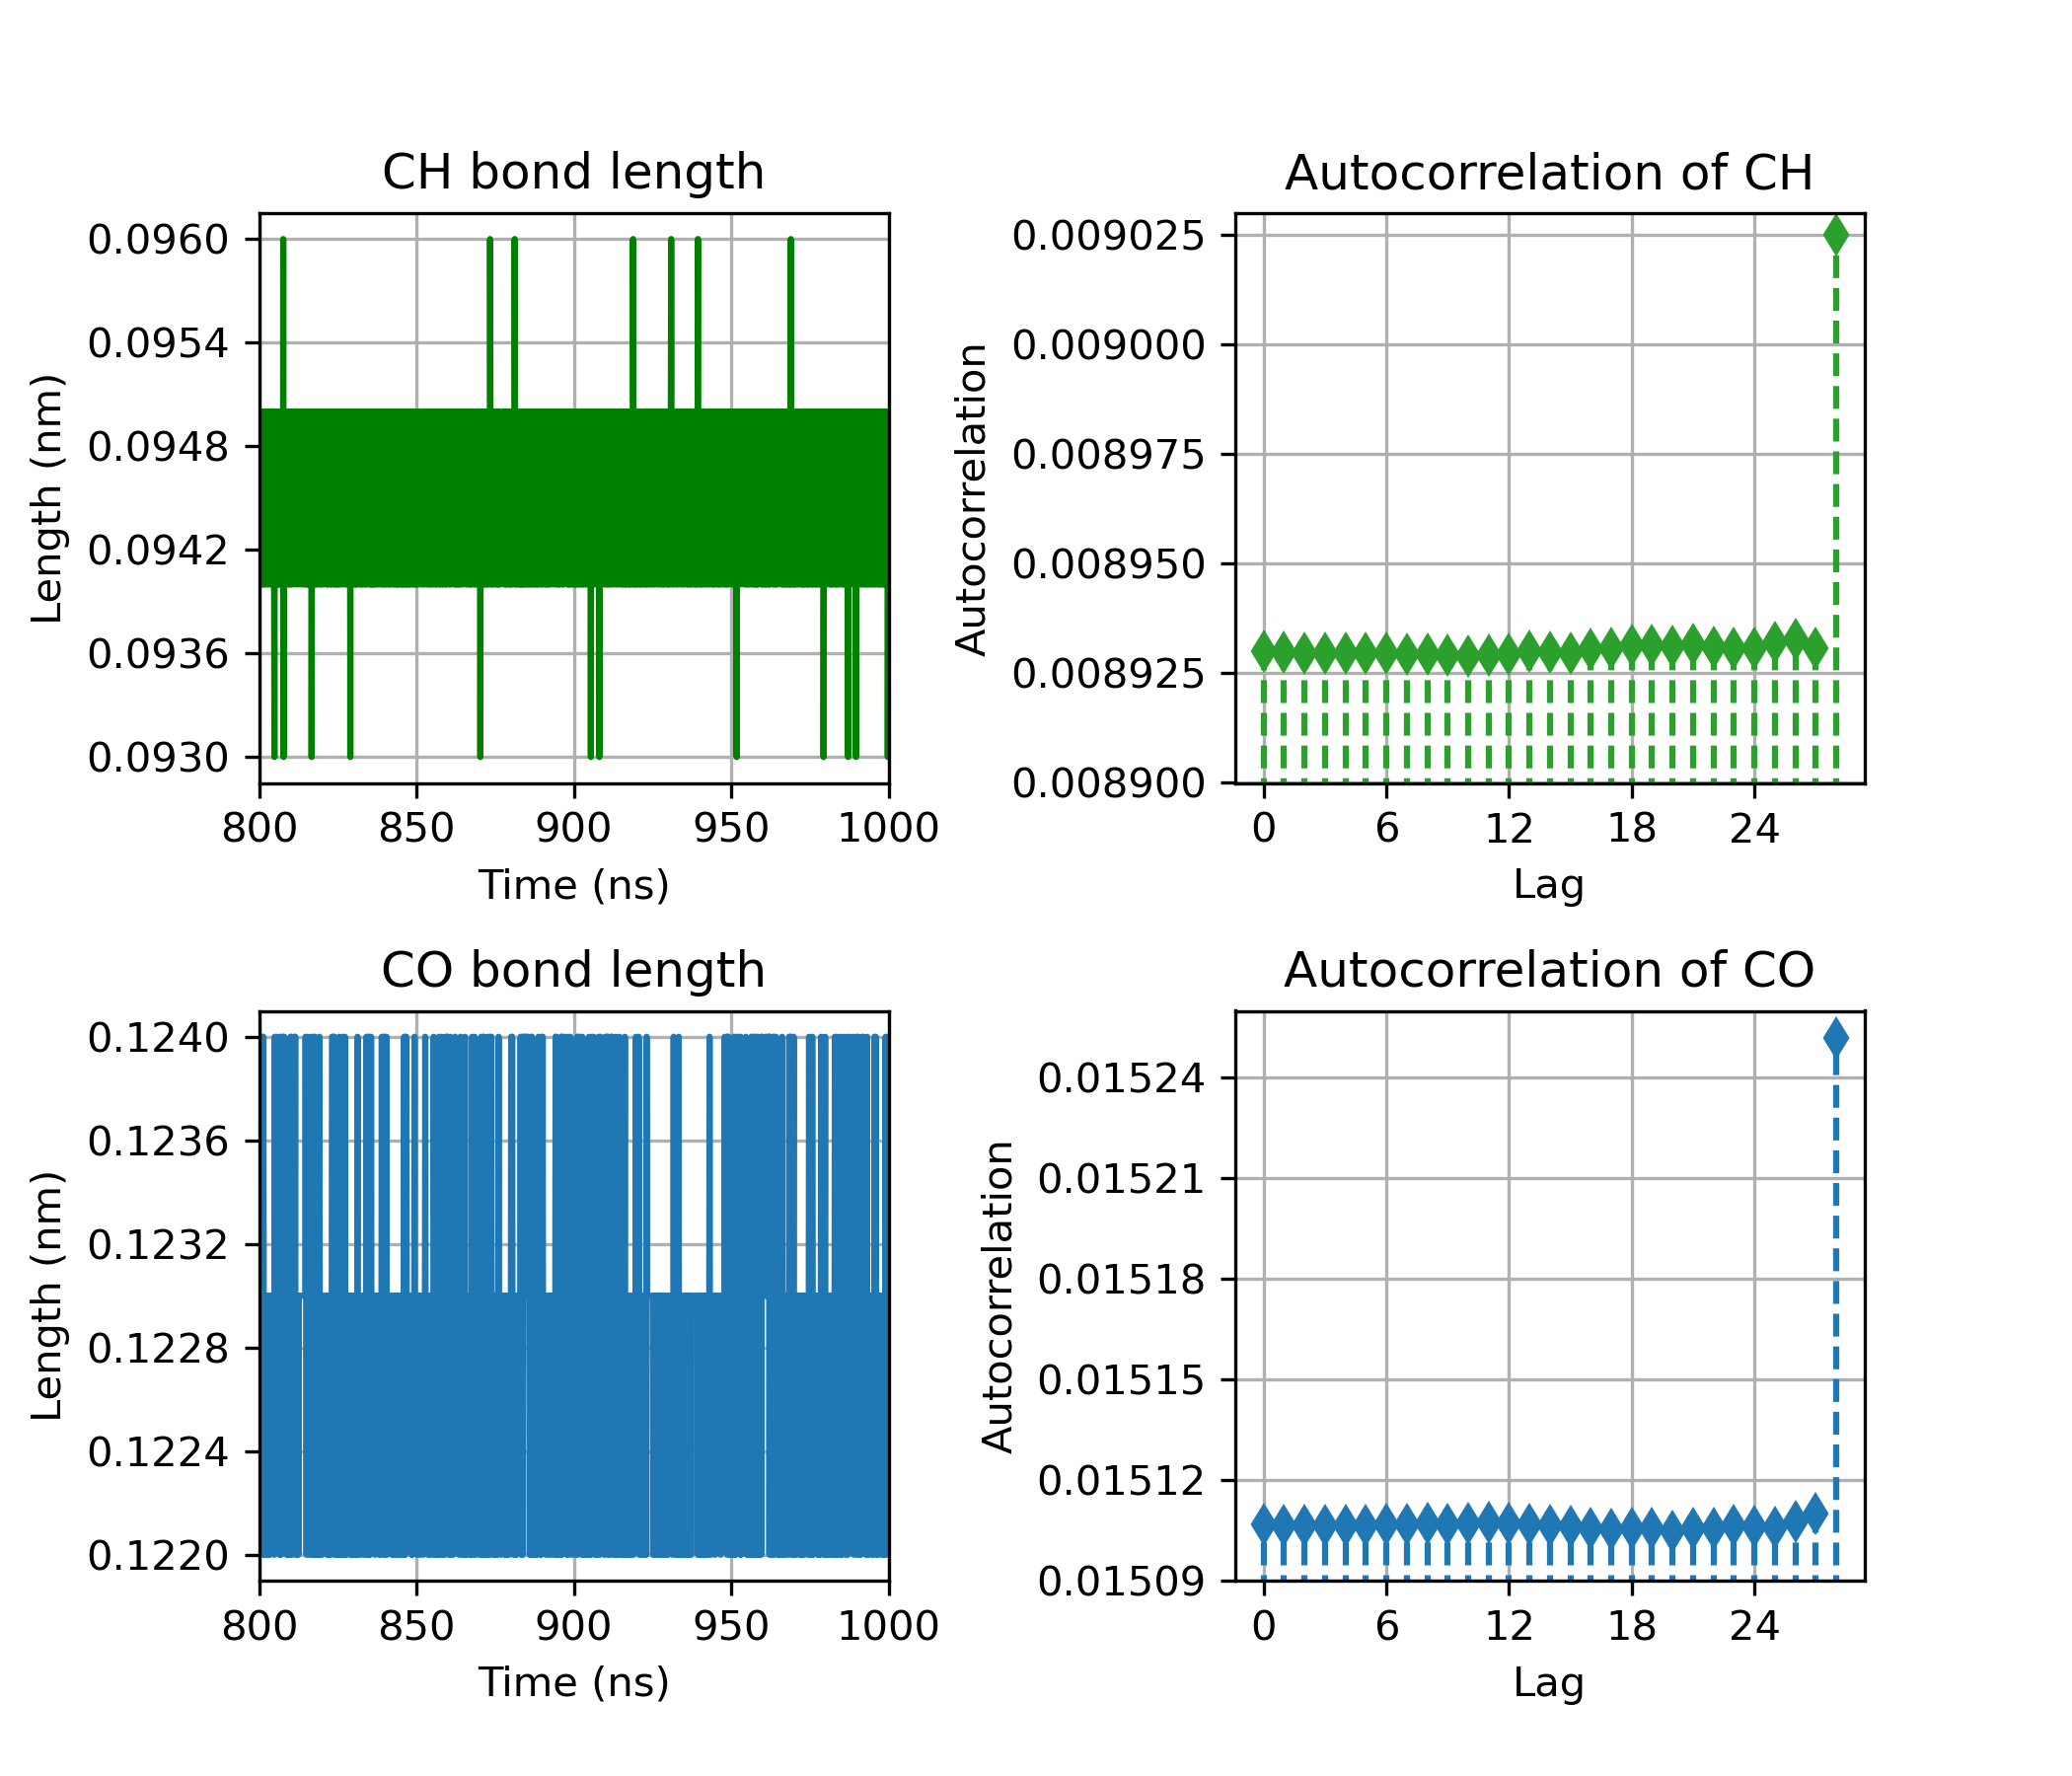
\includegraphics[width=\linewidth]{CO_CH_length_acf_plot.png}
\caption{XXC-H and C=O bond length over Molecular Dynamics time and their autocorrelation function.}
\label{acf_plot}
\end{figure}

\end{task11}


\subsection{Task 2}


Text

\begin{figure}[H]
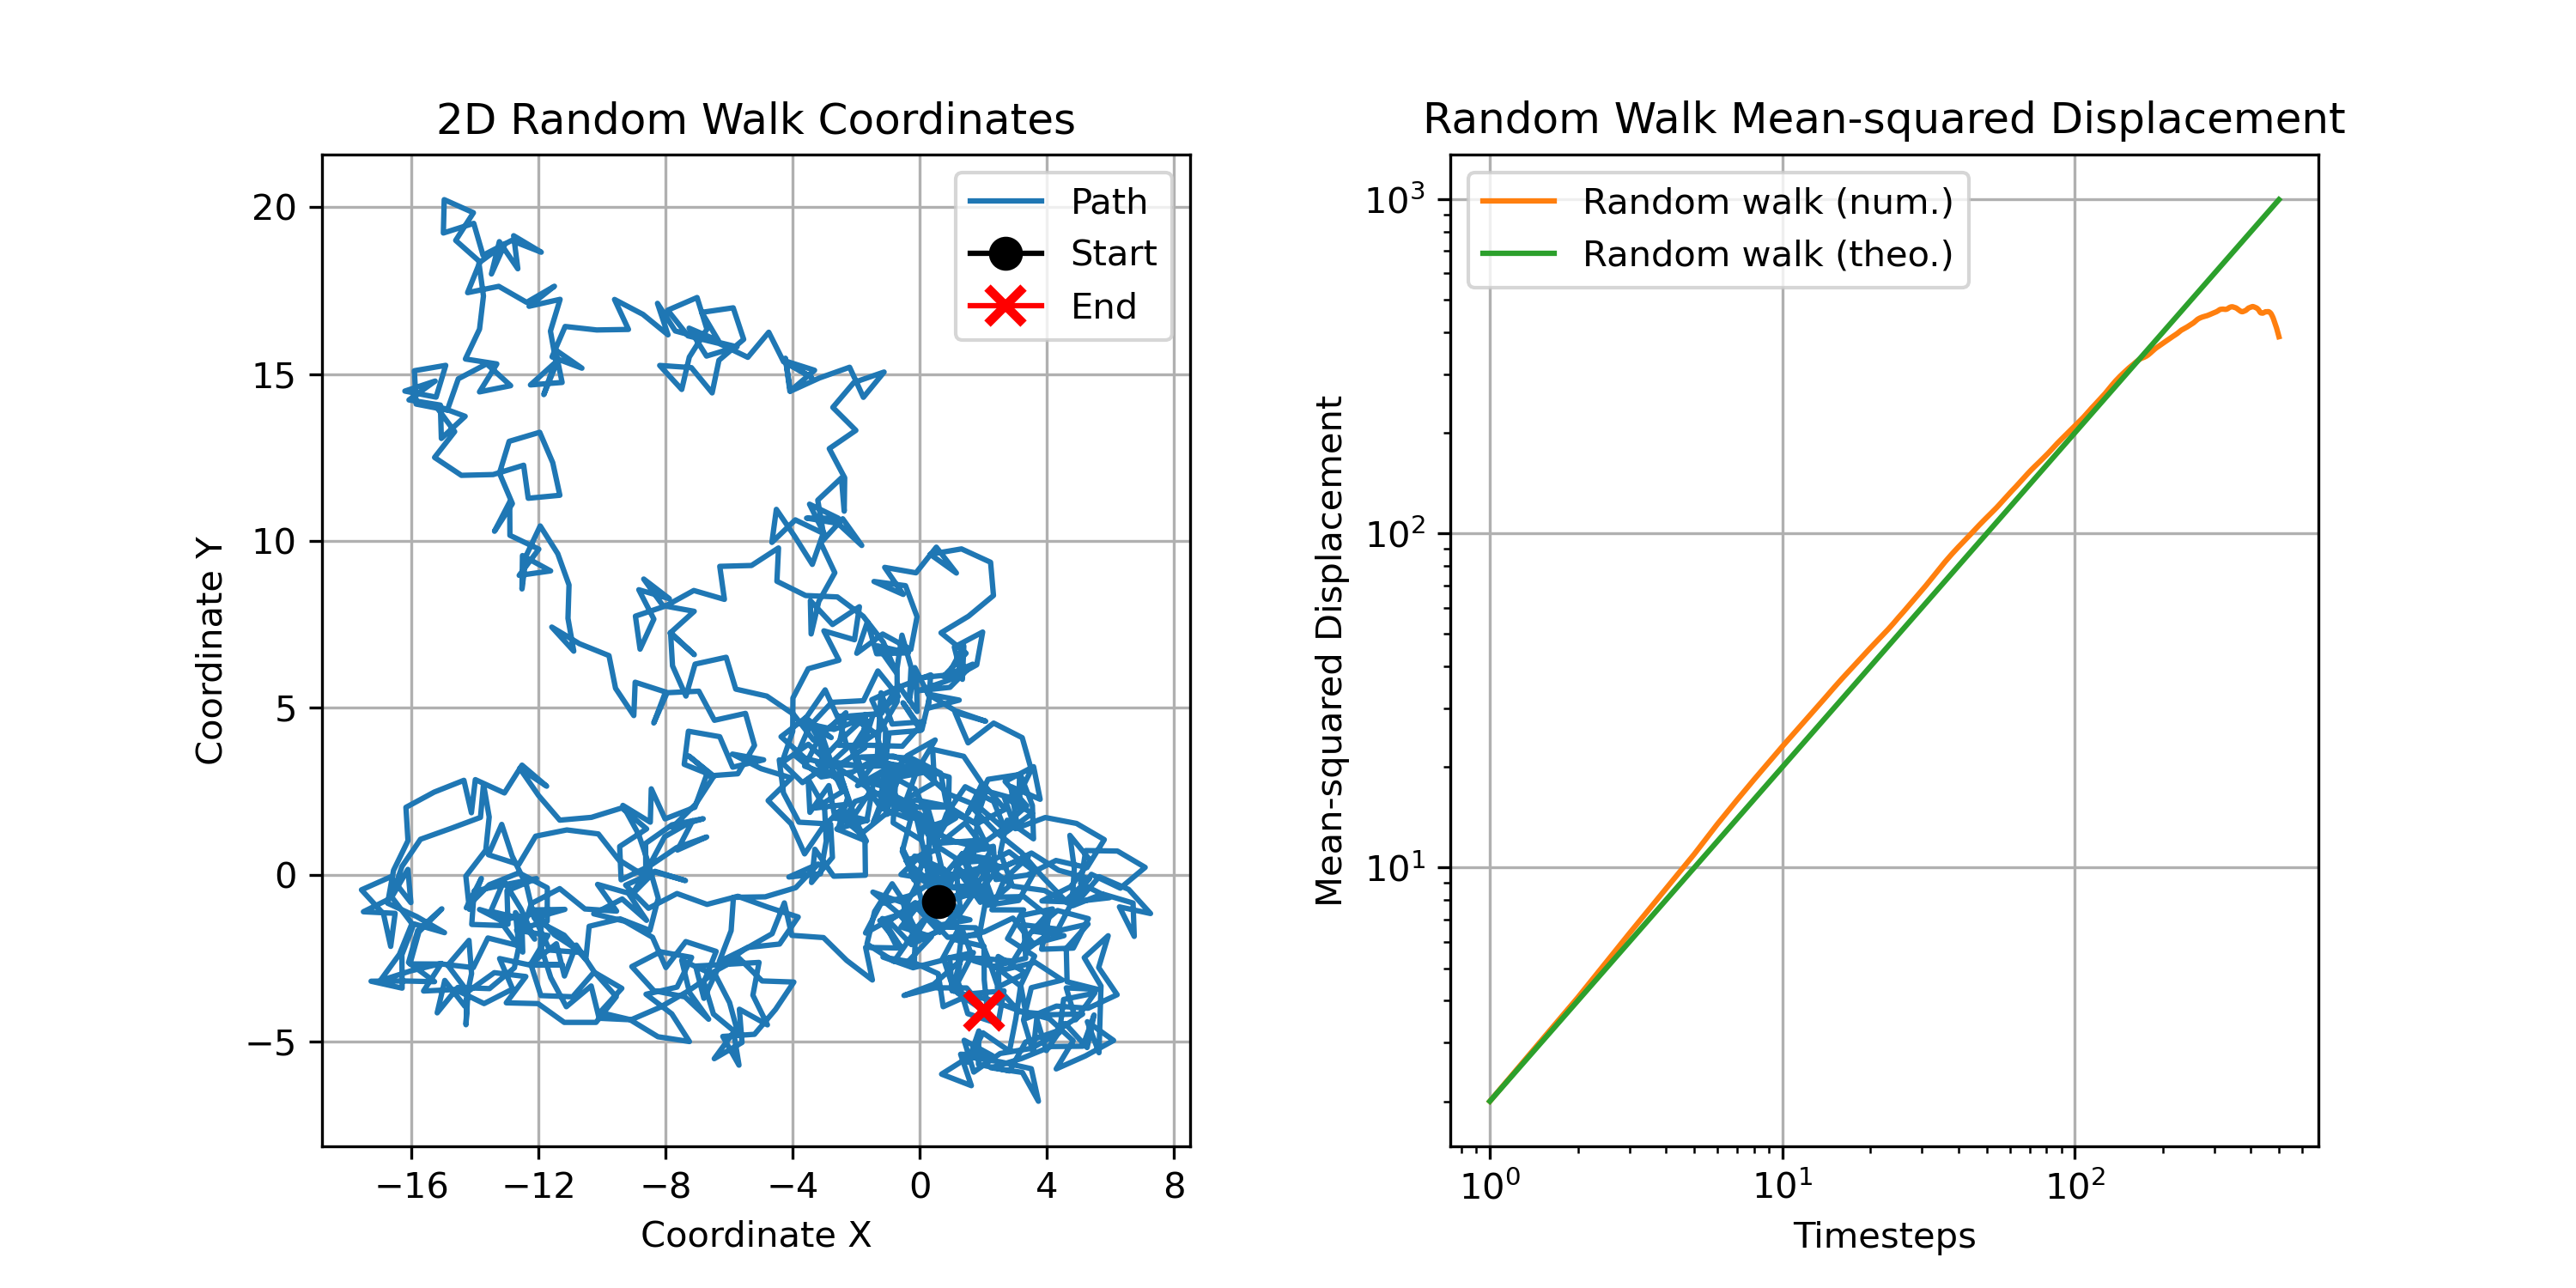
\includegraphics[width=\linewidth]{msd_plot.png}
\caption{2D random walk in a (x,y) coordinates and its mean-squared displacement.}
\label{msd_plot}
\end{figure}



\section{Conclusions}


\bibliography{refs}

\end{document}

\begin{thebibliography}{60}

\bibitem{Hos} de Buyl, Pierre. "tidynamics: A tiny package to compute the dynamics of stochastic and molecular simulations." \it Journal of Open Source Software\rm , 3, no. 28 (2018): 877.

\end{thebibliography}


\end{document}
